%
% 
%
%%%%%%%%%%%%%%%%%%%%%%%%%%%%%%%%%%%%%%%%%%%%%%%%%%%%%%%%%%%%%%%%%%%%%%%%
\chapter{Fundamental Classes in CPPINTS}
%
%
%
In this chapter we will focus on the details on the fundamental classes
in CPPINTS program. They are the bricks for building the recursive
relation.

\section{Basis Set}
%
% 1  what's the form of basis sets?
% 2  why in basis set class we only store l,m,n information?
%
\label{bs}

In quantum chemistry, the basis set functions is the fundamental 
unit for practical calculations\cite{Davidson_Feller_CR_86_681_1986}. 
The basis set functions we discussed here are formed based on Gaussian 
functions as it's radial part, and for the angular part it could be further 
divided into two groups in terms of its function form.  
One group uses the spherical harmonics as shown below:
\begin{equation}
 \chi = Y_{m}^{L}(\theta,\phi)e^{-\alpha r^{2}}
\end{equation}
The other group uses the Cartesian function:
\begin{equation}\label{basis_set_cart_form}
 \chi = x^{l}y^{m}z^{n}e^{-\alpha r^{2}}
\end{equation}
In this program, we only focus on the Cartesian type
Gaussian basis set functions.

Practically, the basis set function $\psi$ is a linear combination of 
Gaussian primitive functions:
\begin{equation}\label{program_contract_basis_set}
	\psi = \sum_{\mu}d_{\mu}\chi_{\mu}
\end{equation}
$d$ is it's contraction coefficients who are pre-optimized 
coefficients. $\chi_{\mu}$ is the primitive 
functions as defined in \ref{basis_set_cart_form}.
All of $\chi$ are on the same center as $\psi$, and they all share the 
same angular momentum with the basis set function.

For each basis set function, $x^{l}y^{m}z^{n}$ is its angular momentum part,
which is characterized by three number of l, m, and n. The $e^{-\alpha r^{2}}$
is its radial part, so l,m,n combined with exponential factor $\alpha$ and 
its coefficient of $d_{\mu}$, that give all of information to get $\psi$.

In the recursive relation, the only thing we cares about 
is the angular part information. As one can see in the recursive
relation, we starts from the bottom integral then by raising up the 
angular momentum we reach the target integrals. Therefore in the basis set class, 
we only use $l,m,n$ to represent the basis set.

In the program we also define the ``NULL'' basis set which means that 
this basis set is physical meaningless (l, m and n are all set to be -1). 
This type of basis set is used to complete an integral definition (see the \ref{integral} 
for more definition).

The basis set is defined in the file basis.cpp and basis.h.

%%%%%%%%%%%%%%%%%%%%%%%%%%%%%%%%%%%%%%%%%%%%%%%%%%%%%%%%%%%%%%%%%%%%%%%%
\section{Shell}
%
% 1  what's the shell? Why shell only have one data member of L?
% 2  what is the basis set order? How can we change it?
%
\label{shell}

In quantum chemistry, shell is an aggregation of same type of basis set
functions; whose total angular momentum is same(sum of l,m,n). For example, 
P shell contains 3 basis set functions, their l, m, n are characterized by:
\begin{align}\label{pshell_example}
	P_{x} &\Leftrightarrow (1,0,0) \nonumber \\
	P_{y} &\Leftrightarrow (0,1,0) \nonumber \\
	P_{z} &\Leftrightarrow (0,0,1)
\end{align}
Therefore, it's able the name the D shell ($L = l+m+n = 2$), 
F shell ($L = l+m+n = 3$) etc.

As what we have demonstrated in the basis set functions section, to use
recursive relation it only requires the angular momentum information. 
Therefore, in the shell class it's only the total angular momentum L
is defined.

Here it needs to emphasize that how to arrange the basis set
functions in a given shell, this is called ``basis set order''.
For example, for the P shell, it's able to have:
\begin{equation}
 P_{x} \Rightarrow P_{y} \Rightarrow P_{z}
\end{equation} 
or the other order of 
\begin{equation}
 P_{z} \Rightarrow P_{y} \Rightarrow P_{x}
\end{equation} 

Since different basis sets in a shell are in a same level, therefore
there's not a basis set order prior to the others. It's able to 
pick up any basis set order theoretically. In this program, we 
pick up the ``libint'' order (which is used by libint program
\footnote{\url{http://sourceforge.net/projects/libint/}}). 
In basisutil.h, the arrangement of basis set order is given for 
L up to 20. On the other hand, it's able to use the other 
type of basis set orders. Therefore we separate the basis set 
order information all into the basisutil.h and basisutil.cpp.

On the other hand, each basis set occupies a unique position in the 
basis set order array, which refers as ``local index'' of the 
basis set in the given shell. For example, in the above P shell
case \ref{pshell_example} $Px$ is 0, $Py$ is 1, $Pz$ is 2. For 
each basis set it's able to set up some ``ONE-TO-ONE'' mapping 
relation between basis set and it's position in the basis set 
order list. Such fundamental relation is also used for the 
mapping between shell quartet and integral.

If the user wants to employ other type of basis set order other 
than the libint order, here is the procedure that should be 
followed:
\begin{itemize}
 \item generate all of explicit basis set order array and 
	 replace the old content of ``LIBINT\_BASIS\_SET\_ORDER''
	 with the new array (this is in basisutil.h). This step
	 will enable you to get correct basis set by given 
	 a basis set index;
 \item Secondly the function of ``getLocalBasisSetIndex'' in
	 basisutil.cpp should be also updated for your new basis 
	 set order. This step will give the correct local index
	 by an arbitrary l, m, n value of basis set.
\end{itemize}
Now the mapping between index and angular momentum should be 
set up. You should get correct integral results without 
referring to the other places.

Similar with basis set, we also define ``NULL'' shell whose 
L is set to be -1. This type of shell is used to complete 
shell quartet definition.

The shell is defined in shell.h and shell.cpp.

%%%%%%%%%%%%%%%%%%%%%%%%%%%%%%%%%%%%%%%%%%%%%%%%%%%%%%%%%%%%%%%%%%%%%%%%
\subsection{Composite Shells}
%
% 1  what is the composite shell?
% 2  how we handle the composite shell? 
\label{composite_shell}
%
%
In quantum chemistry, it's able to construct the composite shells.
The composite shell is that for each shell it may contain several
type of sub-shells. For example, SP shell has one S shell and one 
P shell, and SPD shell has S shell, P shell and a D shell. All of 
these sub-shells share the same exponential factors for radial part,
and each of them has its own contraction coefficients of $d$ in equation
\ref{program_contract_basis_set}. The most famous basis set library using 
composite shell is Pople basis sets (6-31G etc.)

In our program, the shell class is defined for ``pure'' shell and 
the composite shell situation is handled elsewhere. You can refer
to the section \ref{composite_shell_quartet} for more details.

%%%%%%%%%%%%%%%%%%%%%%%%%%%%%%%%%%%%%%%%%%%%%%%%%%%%%%%%%%%%%%%%%%%%%%%%
\section{Integral Type}
%
% how to represent the integral operator?
%
\label{inttype}

In the program, we have a series of pre-defined integer to represent 
the ``OPERATORS'' used in quantum chemistry integrals. For example,
the two body overlap integral, nuclear-electron attraction integral(NAI)
etc. These integers are defined in the inttype.h and inttype.cpp(it's 
name appears as macro defined in general.h). The pre-defined integral 
is a data member for both integral and shell quartet class.

For the given integral type, there are some integral properties that 
is solely determined by the integral operator itself. For example,
NAI is two body integral, and it requires $(0|0)^{(m)}$ calculation etc.
You can find the details from inttype.cpp that what kind of properties 
can be determined only from operator itself.

%%%%%%%%%%%%%%%%%%%%%%%%%%%%%%%%%%%%%%%%%%%%%%%%%%%%%%%%%%%%%%%%%%%%%%%%
\section{Integral and Shell Quartets}
%
% 
%
%%%%%%%%%%%%%%%%%%%%%%%%%%%%%%%%%%%%%%%%%%%%%%%%%%%
\subsection{Integral}
\label{integral}
%
% 1  what is integral?
% 2  how to represent it?
%
For a given operator representing quantum quantity (for example,
the kinetic operator, electron repulsion operator etc.) it's able 
to form the integrals based on the basis set functions:
\begin{equation}
 I = \langle \psi_{l_{1}m_{1}n_{1}}(r)\psi_{l_{2}m_{2}n_{2}}(r)| 
 \hat{f}(r,r^{'})| \psi_{l_{3}m_{3}n_{3}}(r^{'})
 \psi_{l_{4}m_{4}n_{4}}(r^{'})\rangle
\end{equation}
therefore to define an integral, basically you need the following
information:
\begin{itemize}
 \item operator;
 \item basis set information for all given integral positions
\end{itemize}
Because in recursive relation we may need to handle the integrals
of $(ab|cd)^{(m)}$, therefore we have an additional m value defined
in integral class.

Basically, the integrals could be divided into groups according 
to the number of its basis set components. In quantum chemistry, 
the possible number of basis set in the integral could be ranging 
from 1 to 4. Therefore, integrals are ranging from one body integral to 
four body integrals. 

The four possible basis set position are called as: ``BRA1'', ``BRA2'',
``KET1'' and ``KET2''. For one body integral, it's only the bra1
position having basis sets(other positions have null basis set); 
for the two body integral, it's only bra1 and bra2 positions having 
basis sets; for the three body integral, 
it's only bra1, bra2, and ket1 positions having basis sets. 
Such position definition is used across the whole program, and the 
similar definition holds for shell quartet, too.

The integral class always has four position for the basis set (see 
integral.h). For the one to three body integrals, we use NULL
basis set to complete the integral definition.

The integral is defined in integral.cpp and integral.h.
%%%%%%%%%%%%%%%%%%%%%%%%%%%%%%%%%%%%%%%%%%%%%%%%%%%
\subsection{Shell Quartet}
%
% how to define shell quartet?
% what is the relation between shell quartet and integral?
%
\label{shell_quartet}
Similar to the relation between basis set and shell, the aggregation 
of certain type of integrals will lead to the ``shell quartet''.

For example, for the electron repulsion operator it's able to define 
the shell quartet over four shells:
\begin{equation}
 SQ_{P,P,P,P} = \langle P_{bra1}P_{bra2}|
 \frac{1}{r_{12}}|P_{ket1}P_{ket2} \rangle
\end{equation}
This shell quartet includes all of integrals in terms of basis sets
for the given four P shells. Because each P shell have 3 basis set
functions, the shell quartet contains $3^{4} = 81$ ERI integrals.

Similar to the integral class which is defined based on the basis set
class; the shell quartet is constructed based on the shell class. Therefore
for defining a fundamental shell quartet, you need shell information
on all of four BRA1, BRA2, KET1 and KET2 positions (null shell is used
to complement the shell quartet definition) as well as the operation
information.

The definition of shell quartet could be referred to shellquartet.h
and shellquartet.cpp.

%%%%%%%%%%%%%%%%%%%%%%%%%%%%%%%%%%%%%%%%%%%%%%%%%%%
\subsection{Mapping between Integral and Shell Quartet}

For this program, shell quartet is the basic unit for deriving the 
recursive relation. The integrals are considered to be attached to 
its corresponding shell quartet.

Based on the ``ONE-TO-ONE'' mapping relation between basis set 
and shell, it's able to construct the ``ONE-TO-ONE'' mapping relation
between integral and its shell quartet. For each integral, it 
has a unique position according to the given basis set order.
For example, integrals in the shell quartet $(SPSP|SPSP)$ may 
correspond to an order like:
\begin{align}
 (SS|SS)         &\rightarrow  0 \nonumber \\
 (P_{x}S|SS)     &\rightarrow  1 \nonumber \\
 (P_{y}S|SS)     &\rightarrow  2 \nonumber \\
 (P_{z}S|SS)     &\rightarrow  3 \nonumber \\
 (SP_{x}|SS)     &\rightarrow  4 \nonumber \\
 (P_{x}P_{x}|SS) &\rightarrow  5 \nonumber \\
 (P_{y}P_{x}|SS) &\rightarrow  6 \nonumber \\
 (P_{z}P_{x}|SS) &\rightarrow  7 \nonumber \\
                 &\cdots
\end{align}
By giving the shell quartet and this unique position, it's able 
to reconstruct the integral; on the other hand, from the given 
integral it's able to derive its unique position\footnote{please
refer to integral.cpp for more details that how we do it}.

%%%%%%%%%%%%%%%%%%%%%%%%%%%%%%%%%%%%%%%%%%%%%%%%%%%
\subsection{Representation of Integral in Recursive Relation}
%
% why we use position ID to reprernt integral in shell quartet?
%
\label{representation_integral_sq}

The ``ONE-TO-ONE'' mapping relation could be used to improve the memory 
usage for this program. Suggest we have a $(II|II)$ ERI shell 
quartet for deriving its vertical recursive relation (assume
that we are under OS VRR framework), to record
all of the information for each integrals requires the following 
items:
\begin{itemize}
 \item LHS integral;
 \item RHS integral and its coefficients.
\end{itemize}

For each integral, to characterize it it requires $3\times 4 = 12$
integers to record angular momentum information, plus two integers
for operator and m value. Therefore each integral needs 14 integer
\footnote{we have not considered the division yet, which is related to
composite shell quartet case}.

For the OS VRR framework, the recursive relation has 8 items on the 
RHS so there are totally 9 integrals, which needs 126 integers. 
Because the $(II|II)$ has $28^4$ integrals, it needs 77446656 integers.
Suggest each integer takes 4 byte memory, the total memory for 
storing integer of this shell quartet would be 296mb! So far we did not
count in the coefficients.

However, if we use the ``position ID'' to represent the integrals 
inside the shell quartet, then each integral only need one integer 
thus it's only 5.3mb memory needed. Therefore, to use the position 
ID to represent integrals inside shell quartet is a good way for 
memory saving with only marginal CPU cost added. This is the way
we handle integrals in the recursive relation(RR) process.

%%%%%%%%%%%%%%%%%%%%%%%%%%%%%%%%%%%%%%%%%%%%%%%%%%%
\subsection{Composite Shell Quartet}
%
%
\label{composite_shell_quartet}

In a given shell quartet, if one of its shell is in composite type; 
then this shell quartet is composite shell quartet. It contains
several shell quartets in terms of pure shell. For example,
shell quartet $(DD|DSP)$ has two pure shell quartets; namely 
$(DD|DS)$ and $(DD|DP)$.

How to process composite shell quartet in the recursive relation?
It's depending on whether it's HRR or it's in VRR.

For VRR, Let's take ERI as example. Because the recursive relation 
is generally expressed as: 
\begin{align}
I(L,m) &= a_{0}I_{0}(L-1,m) + a_{1}I_{1}(L-1,m+1) \nonumber \\ 
&+ a_{2}I_{2}(L-2,m) - a_{3}I_{3}(L-2,m+1) \nonumber \\
&+ a_{4}I_{4}(L-2,m) - a_{5}I_{5}(L-2,m+1) \nonumber \\
&+ a_{6}I_{6}(L-2,m+1) + a_{7}I_{7}(L-2,m+1)
\end{align}
The above integral expression is on primitive Gaussian function, and 
$a_{i}$ is coefficient which is independent with the integral.
Because VRR is linear with the contraction coefficients $d$,
the expression above holds for contracted or un-contracted primitive
Gaussian functions. Therefore, the recursive relation for VRR is 
independent of the contraction information. We can simply get the 
integral with contraction coefficients by multiply it to the final
results:
\begin{equation}\label{composte_sq_contraction_coefs}
 I_{contracted}(L,m) = d_{bra1}d_{bra2}d_{ket1}d_{ket2}I(L,m)
\end{equation}
This is what we do for dealing with the composite shell quartets.
Because in composite shell the sub-shells share the same exponential
factor, the raw integral $I(L,m)$ in \ref{composte_sq_contraction_coefs} 
is same for different pure shell quartets; the final integral results
with contraction coefficients could be simply retrieved by performing 
\ref{composte_sq_contraction_coefs}. This is called ``contraction'' step
in VRR. The pseudocode is given like this:
\begin{verbatim}
loop over ket side primitive Gaussian pairs:
  loop over bra side primitive Gaussian pairs:
    compute bottom integrals;
    do VRR to derive result integrals;
    perform contraction step; 
  end loop
end loop
\end{verbatim}
For pure shell quartet like $(DD|DD)$, we have no need to perform 
contraction step because we can simply add contraction information
to the bottom integrals $(00|00)^{(m)}$ so that VRR is performed 
for contracted integrals. After VRR is ending, we just simply update
the results.

However, for HRR things are different. Because HRR is usually applied on
contracted integral results (it sums over all of integrals on 
primitive Gaussian functions), we can see that how we can step from
un-contracted integrals to contracted ones in HRR:
\begin{align}\label{composite_sq_hrr}
 [a(b+\iota_{i})|cd]_{k} &= [(a+\iota_{i})b|cd]_{k} + 
(A_{i} - B_{i})[ab|cd]_{k} \rightarrow \nonumber \\
\sum_{k}C_{k}[a(b+\iota_{i})|cd]_{k} &= \sum_{k}C_{k}[(a+\iota_{i})b|cd]_{k} + 
(A_{i} - B_{i})\sum_{k}C_{k}[ab|cd]_{k} \rightarrow \nonumber \\
(a(b+\iota_{i})|cd) &= ((a+\iota_{i})b|cd) + 
(A_{i} - B_{i})(ab|cd)
\end{align}
Here we use $[ab|cd]$ to represent the integrals on un-contracted Gaussian 
functions, and $(ab|cd)$ for the contracted integrals; $C_{k}$ is the 
combination for all of contraction coefficients of $d$.

It's clear from \ref{composite_sq_hrr} as long as LHS and RHS share the 
same contraction coefficients, HRR can be applied from $(0e|0f)$ until
we get the final target integral $(ab|cd)$. Hence for the composite 
shell quartets, each pure shell quartet has its own HRR process and they
are independent with each other.

For this reason, we have a data member named as ``division'' on both
integral and shell quartet classes. It's an ID for each pure shell quartet
in the composite one, for example; for $(DSP|DSP)$ it has four shell quartets;
$(DS|DS)$, $(DS|DP)$, $(DP|DS)$ and $(DP|DP)$ and each one has it's 
own ID number (characterized by division). They will have their own
HRR process.

%%%%%%%%%%%%%%%%%%%%%%%%%%%%%%%%%%%%%%%%%%%%%%%%%%%
\subsection{Sorting of Shell Quartets in RR}
%
%



%%%%%%%%%%%%%%%%%%%%%%%%%%%%%%%%%%%%%%%%%%%%%%%%%%%%%%%%%%%%%%%%%%%%%%%%
\chapter{Core Concepts of CPPINTS}

\section{Introduction}
\label{concepts_introduction}

The integral we discussed here is analytical integrals,
which is generally expressed as:
\begin{equation}\label{int_paper:1}
  I_{ijkl} = \int \chi_{i}(\bm{r})\chi_{j}(\bm{r})f(\bm{r},\bm{r^{'}})
\chi_{k}(\bm{r^{'}})\chi_{l}(\bm{r^{'}}) d\bm{r} d\bm{r^{'}}
\end{equation}
and the integrand is analytically integrated. Kinetic integrals(KI),
nuclear attraction integrals(NAI), electron repulsion integrals(ERI) etc. all 
belong to this group. 

Since Boys\cite{SFBoys1950} suggested to use Cartesian Gaussian type function to form 
basis functions,
\begin{equation}\label{int_paper:2}
 \chi = x^{i}y^{j}z^{k}e^{-\alpha r^{2}}
\end{equation}
a major breakthrough technology for computing ERI was introduced by Pople and Hehre(PH)\cite{PH}. 
This method provides exceptional efficient algorithm for computing high contracted 
low angular momentum integrals. However, this method is limited to S and P basis functions, 
and it's difficult to be extended to high angular momentum integrals. McMurchie and Davidson(MD)\cite{MD}
proposed a general formalism for computing variety kind of analytical integrals in terms of 
Hermitian polynomials, and their method is applied to integrals with high angular momentum. 
Dupuis, Rys and King(DRK)\cite{DRK1976JCOMP,DRK1976JCP,DRK1983JCOMP} developed another formalism 
for ERI based on exact numerical 
quadrature using root and weights generated from Rys polynomials. Although MD and DRK
methods provide general way to derive the analytical integrals, they are indirect methods where
auxiliary polynomials need to be involved. 

In 1980s, Obara and Saika(OS)\cite{OS1986,OS1988} derived a set of
recursive formulas for analytical integrals based on recursive expression of 
three body overlap integral. In the OS method it's able to directly generate the integrals. The 
recurrence relation(RR) for ERI in OS scheme is given as:
\begin{equation}
 \begin{split}
((a+\iota_{i})b|cd)^{(m)} &= (P_{i} - A_{i})(ab|cd)^{(m)} +
\left(W_{i} -P_{i}\right)(ab|cd)^{(m+1)} \\
&+\frac{N_{i}(A)}{2\epsilon}\left(((a-\iota_{i})b|cd)^{(m)}-\frac{\rho}{
\epsilon }((a-\iota_{i})b|cd)^{(m+1)}\right)  \\
&+\frac{N_{i}(B)}{2\epsilon}\left((a(b-\iota_{i})|cd)^{(m)}-\frac{\rho}{
\epsilon }(a(b-\iota_{i})|cd)^{(m+1)}\right)  \\
&+\left(\frac{N_{i}(C)}{2}\right)\frac{1}{\epsilon+\eta}
(ab|(c-\iota_{i})d)^{(m+1)} \\
&+\left(\frac{N_{i}(D)}{2}\right)\frac{1}{\epsilon+\eta}
(ab|c(d-\iota_{i}))^{(m+1)}
\end{split}
\label{int_paper:3}
\end{equation}
where the $(ab|cd)^{(m)}$ is:
\begin{equation}
\label{int_paper:4}
 (ab|cd)^{(m)} = \frac{2}{\sqrt{\pi}}\int^{\infty}_{0} du \left( \frac{u^{2}}
{\rho+u^{2}}\right)^{m}(ab|u|cd) 
\end{equation}
$(ab|cd)^{(0)}$ is the result ERI of $(ab|cd)$. In the OS scheme to compute an arbitrary ERI 
of $(ab|cd)$, the bottom integrals of $(00|00)^{(0)}$, $(00|00)^{(1)}$ etc. are needed 
to be evaluated first; through the recursive expansion \ref{int_paper:3} it's able to raise
up the angular momentum recursively until the target integral $(ab|cd)$ is derived. Lindh, 
Ryu and Liu\cite{lindh1991reduced}(LRL) proposed a similar RR based on Rys 
polynomials. Because the integrals are calculated in ``vertical'' way, 
such methods are named as ``vertical recurrence relation''(VRR).

In contrast to the VRR, Head-Gordon and Pople(HGP)\cite{HGP} found another general formula which 
performs ``horizontal recurrence relation''(HRR) on analytical integrals. In HRR the ERI
is evaluated as:
\begin{equation}
\label{int_paper:5}
 (a(b+\iota_{i})|cd) = ((a+\iota_{i})b|cd) + 
(A_{i} - B_{i})(ab|cd)
\end{equation}
Consequently the ERI $(ab|cd)$ can be recursively derived from a set of auxiliary integrals
in form of $(e0|f0)$. Because the HRR only involves the basis function centers,
it can be applied to contracted integrals thus to save computation cost 
inside the contraction loop. Hamilton and Schaefer\cite{new_hrr_Schaefer}(HS) derived a 
similar HRR by using translational invariance condition, it shifts the integral in form of 
$(a+b+c+d0|00)$ to $(a+b0|c+d0)$. 

For practical integral evaluation, HRR needs to combine with other
methods to finish the whole integral derivation. HGP\cite{HGP} scheme combines the HRR with OS scheme,
Gill etc. \cite{gill1989efficient, gill1990efficient}suggested to join HRR and MD methods together. 
Other type of combinations are also proposed\cite{lindh1991reduced,new_hrr_Schaefer}.

Although VRR provides clear formalism for recursively generating integrals, it's still 
uncertain that how to generate the integrals with least amount of work. This problem is 
referred as ``tree-search problem''\cite{HGP}. Generally in the VRR, the recurrence derivation on 
ERI forms a ``directed graph'' data structure\footnote{see 
\url{http://en.wikipedia.org/wiki/Directed_graph} for more details} as shown in figure \ref{fig:1}. The 
tree-search problem is to find the optimal directed graph(or commonly referred as path) with 
minimum of work, for example; with minimum FLOPS or with minimum number of intermediate variables. 

 \begin{figure}[htb]
 \centering
 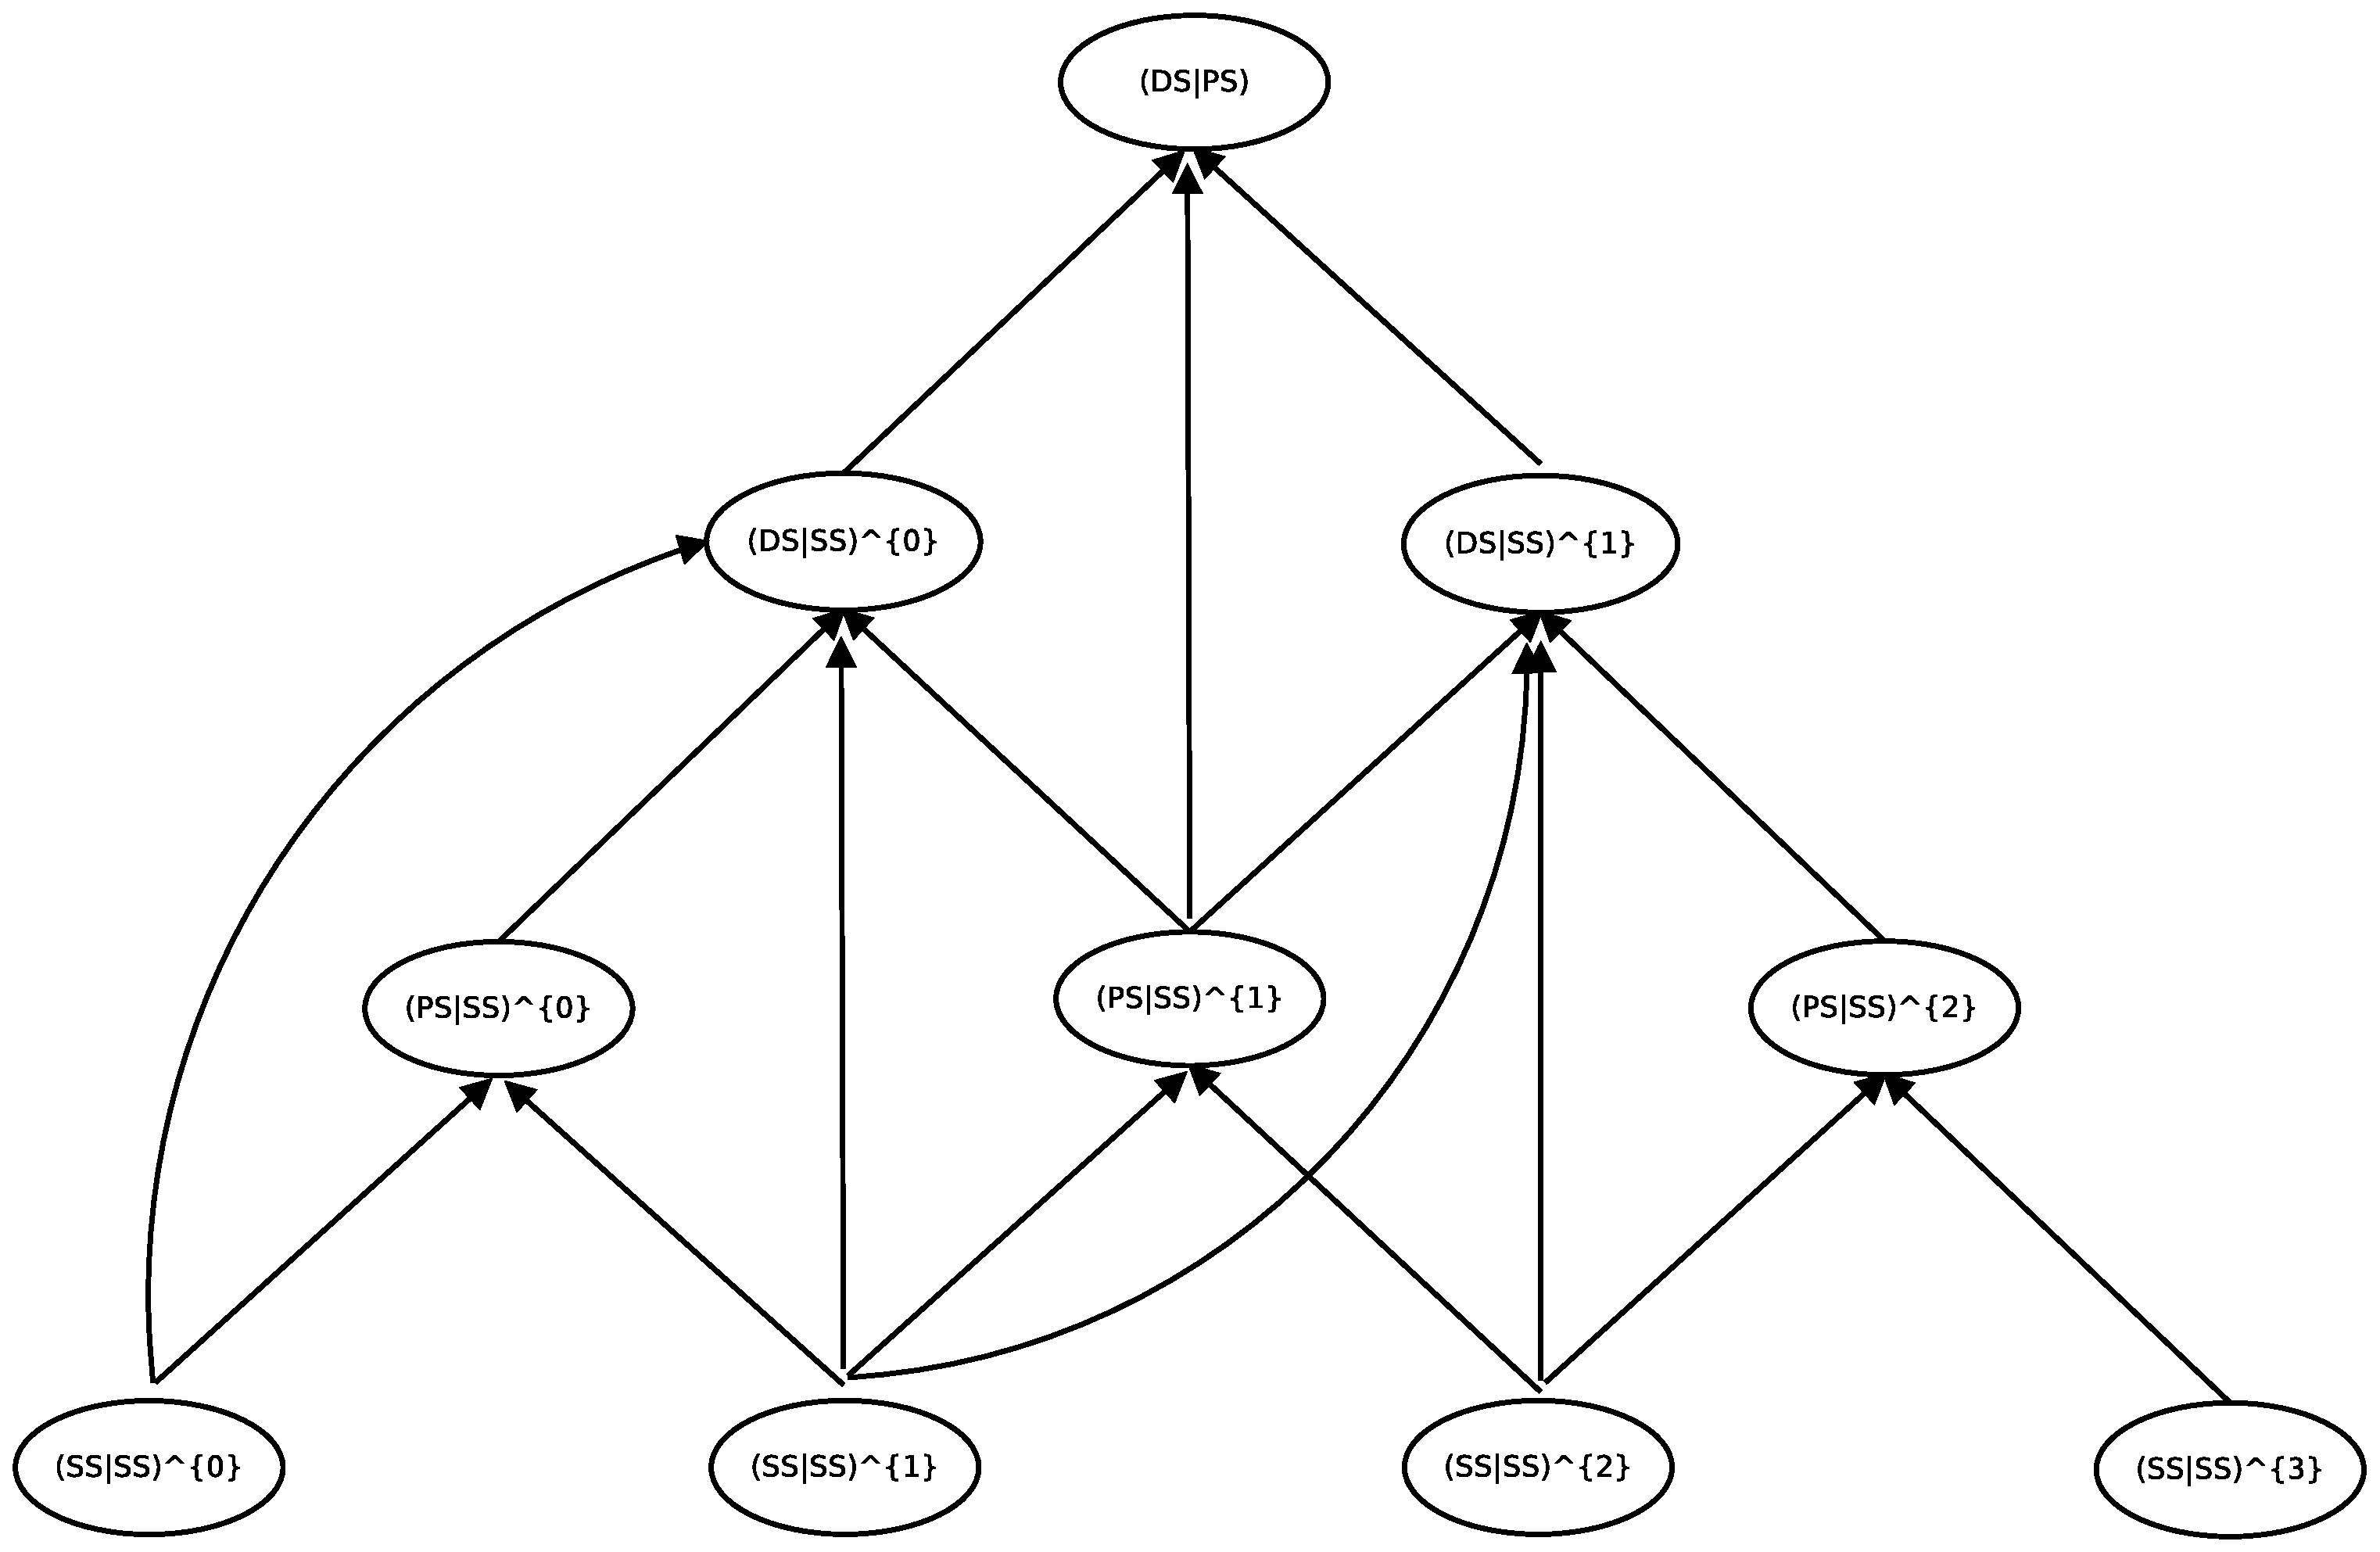
\includegraphics[scale=0.25]{./graph.eps}
 % general_rr.eps: 0x0 pixel, 300dpi, 0.00x0.00 cm, bb=0 0 763 487
 \caption{directed graph for integral of $(DS|PS)$ based on OS scheme}
 \label{fig:1}
\end{figure}

In CPPINTS, a general searching algorithm is used on solving the tree-search problem for 
VRR. Instead of exploring details for optimal path, by
investigating the nature of VRR formula we can wrap up correlated integrals into packages
and it turns out that the packages are independent with each other on the VRR path. Based on
the concept of package, the directed graph for VRR is converted into tree data structure and the optimal
path for VRR is corresponding to the shortest path in the given tree data structure, where the
a similar Dijkstra's algorithm\footnote{please see 
\url{http://en.wikipedia.org/wiki/Dijkstra\%27s_algorithm} for more information} is applied.

For computing the target integrals, both VRR and HRR need many intermediate integrals on
the recurrence relation(RR) path. The interesting question is, is every intermediate integral 
necessary in the recurrence generation? The question becomes more interesting in terms of 
the redundancy of Cartesian type of Gaussian functions in comparison with the spherical form of 
Gaussian functions. In the end of section \ref{optimal_path} a general recursive procedure is 
employed to explore the redundancy of RR.


%%%%%%%%%%%%%%%%%%%%%%%%%%%%%%%%%%%%%%%%%%%%%%%%%%%%%%%
% optimal VRR path
%%%%%%%%%%%%%%%%%%%%%%%%%%%%%%%%%%%%%%%%%%%%%%%%%%%%%%%
\section{Finding Optimal Path for Recurrence Relation}
\label{optimal_path}

The optimal path for RR can be defined in variety of way. In this paper,
the optimal path is the implementation of RR with minimum intermediate integral
number. Our discussion below is based on HGP scheme above. However,the idea 
and implementation below is easy to transfer to other RR schemes.

In the practical implementation of RR, the integral calculation is usually performed 
in terms of shells rather than basis functions, so that to reduce the repeat use of 
intermediate integral. Considering the equation \ref{int_paper:3}, 
all of shell positions in the shell quartet $(FD|PS)$ are expandable except the ``ket2'' position 
where the shell is ``S'' type of 
function. Therefore for each LHS ERI appearing in the VRR, how to find it's proper expandable
position so that to minimize the total number of intermediate integrals is the key to 
find optimal path for VRR.

Let's take ERI as an example. The equation \ref{int_paper:3} can be generalized into a 8-term 
expansion:
\begin{align}\label{int_paper:7}
I(L,m) &= a_{0}I_{0}(L-1,m) + a_{1}I_{1}(L-1,m+1) \nonumber \\ 
&+ a_{2}I_{2}(L-2,m) - a_{3}I_{3}(L-2,m+1) \nonumber \\
&+ a_{4}I_{4}(L-2,m) - a_{5}I_{5}(L-2,m+1) \nonumber \\
&+ a_{6}I_{6}(L-2,m+1) + a_{7}I_{7}(L-2,m+1)
\end{align}
$L$ is the sum of angular momentum
\begin{equation}\label{int_paper:8}
 L = L_{a} + L_{b} + L_{c} + L_{d}
\end{equation}
for ERI $(ab|cd)$, and $m$ is the parameter for auxiliary integral $(ab|cd)^{(m)}$ in 
expression \ref{int_paper:4}.
From equation \ref{int_paper:7}, it's clear that the $L$ is constantly decreasing and $m$ is
increasing in same manner from LHS to RHS. Therefore the properties of $L$ and $m$ 
for ERI characterize an ``arrow'' in the derivation of VRR, in this sense the VRR
for ERI is ``inconvertible'' between LHS and RHS. As see in the following discussion,
such inconvertibility grantees the existence of conversion for transforming the graph
data structure into the tree data structure for ERI\footnote{In tree data structure,
every children node can only have one parent node. Such character establishes the direction
of the tree. Please see \url{http://en.wikipedia.org/wiki/Tree_\%28data_structure\%29} for 
more information}, and it also establishes an order 
of sequence between two arbitrary ERI so that RHS ERI is always generated prior to
the LHS ERI in the resulting VRR path.

Based on the feature of inconvertibility, it's able to set up some general coding structure
to perform the optimal path search for ERI in VRR (unsolved shell quartets are these who
appear in VRR path but their expanding position are not yet determined):
\begin{verbatim}
set up unsolved shell quartet archive;
initilize the unsolved shell quartet archive with 
input LHS shell quartets;
loop over m (from m=0 to maximum):
  loop over L (from maximum to 0):
    while(true):
      perform optimal expanding postion search for 
      all (L,m) LHS shell quartets in the unsolved 
      shell quartet archive;
      if there are no (L,m) LHS shell quartets break 
      out the loop;
    end while
  end loop with L
end loop with m
\end{verbatim}
The search is carried out from the LHS to RHS until all of LHS shell quartets 
are solved. The procedure here establishes a general Dijkstra algorithm scheme 
for searching expanding positions for VRR. By wrapping up all of unsolved 
$(L,m)$ shell quartets together, it's able to search their their optimal expansions
and the following search iteration will be performed based on the output of
previous iterations. 

How to evaluate the efficiency of the algorithm comparing with Breadth-first search
or Depth-first search across all of possible VRR paths? In general the Dijkstra algorithm
can not guarantee a global minimum because the global minimum may not be reached by
by assembling minimums on the partial path. However, because L is constantly decreasing
from LHS to RHS; the integral numbers are constantly decreasing from current search
iteration to the following ones. Therefore it could expect that the above procedure
may give the close VRR path comparing with the global optimum.

In terms of an arbitrary given unsolved $(L,m)$ shell quartets, all of shell quartets
appearing in VRR can be divided into three groups:
\begin{itemize}
 \item unsolved main list;
 \item correlated list;
 \item irrelevant list 
\end{itemize}
Unsolved main list contains the unsolved shell quartets with given properties of $(L,m)$.
Their expanding position are going to be determined in the current iteration of search. 
Correlated list is composed by the unsolved shell quartets who possibly share the RHS 
terms with the unsolved main list. The irrelevant list is composed by all of other 
unsolved shell quartets and their expansion positions are independent with the 
unsolved main list. By combining the unsolved main list and correlated list together 
to form a package, all of correlated LHS shell quartets are self-contained therefore 
it's able to carry out a full search on all possible expansion combinations for every 
LHS shell quartets inside the package. The search result gives the final expanding
positions to the unsolved main list.

Let's take ERI as illustration. The VRR in equation \ref{int_paper:7} demonstrates that 
for ERI $I(L,m)$, only ERI of $I(L-1,m)$, $I(L,m+1)$ and $I(L-1,m+1)$ can share RHS with it.
These ERI are in unsolved state and their undetermined expansion will affect the determination 
of expanding position for $I(L,m)$. On the other hand, although ERI with $L+1$ or $m-1$ are 
also possibly sharing RHS with $I(L,m)$, their expanding position have been solved in previous 
iteration; therefore these shell quartets apply deterministic effects on the search of expanding 
position searching for ERI $I(L,m)$. As a result of inconvertibility of VRR, the number of shell
quartets which constitutes the correlated package decreases significantly.

In summary, for searching the expanding position of shell quartets with property of $(L,m)$, 
it's able to form an independent package with unsolved shell quartets characterized by property 
$(L-1,m)$, $(L,m+1)$ and $(L-1,m+1)$. A complete survey to find minimum RHS integrals for $(L,m)$
shell quartets is performed in terms of all of possible expansion combinations for all of shell 
quartets inside the package. The implementation for the above algorithm is depicted as below:
\begin{verbatim}
set up archive for solved shell quartets;
set up archive for unsolved shell quartets;
initilize the unsolved archive with input shell quartets;

loop over m (from m=0 to maximum):
  loop over L (from maximum to 0):
    while(true)
      construct empty main shell quartet list, and fill 
      in shell quartets with (L,m) from unsolved archive;
    
      construct empty correlated shell quartet list, and 
      fill in possible shell quartets with (L-1,m), 
      (L,m+1) and (L-1,m+1) from unsolved archive;
      
      combine the main shell quartet list and appended
      shell quartet list together into full list;
      
      loop over all possible expanding combinations:
         compare the new RHS shell quartets with solved
         and unsolved archives, remove the new RHS shell
         quartet if it's double couting (vertical 
         comparison);
         
         compare the new RHS shell quartets with each 
         other and wipe out the repeat ones (horizontal
         comparison);
         
         count the number of integrals from all remaining 
         RHS shell quartets, replace the old expansion
         plan with new one if it's outperformed;
      end loop of expanding combination 
       
      for the optimal expansion plan, push the main
      shell quartets into solved archive and the new
      RHS shell quartets into unsolved archive;
       
      is there remaining shell quartets with property
      of (L,m) in unsolved archive?
      if not, step out the while loop;      
    end while
  end loop with L
end loop with m 
\end{verbatim}

The procedure establishes the result VRR path by assemble global minimum on each partial VRR
path along the searching iterations. Such pseudocode not only applies to ERI, but also to
KI, NAI etc. as long as the integral can be derived from recurrence relation with inconvertible
property. Unfortunately, HRR can not employ the above algorithm because the inconvertibility 
is destroyed inside HRR:
\begin{align}
\label{int_paper:9}
 (a(b+\iota_{i})|cd) &= ((a+\iota_{i})b|cd) + AB_{i}(ab|cd)   \nonumber \\
                     &\Updownarrow                            \nonumber \\
 ((a+\iota_{i})b|cd) &= (a(b+\iota_{i})|cd) - AB_{i}(ab|cd)   
\end{align}
For example, if LHS shell quartet $(FD|PS)$ is expanded in terms of shell D position according 
to equation \ref{int_paper:9}, in search of expanding position of result RHS shell quartet $(GP|PS)$
it will resort to the expansion on shell G because the previous LHS $(FD|PS)$ becomes the RHS for
expanding $(GP|PS)$ and $(FD|PS)$ is already contained in the result path. As a result, the expansion 
search forms a cycles and the expanding positions for LHS shell quartets are never to be correctly 
determined in the generated HRR path.

In HRR we use another way to determine the optimal path. Since HRR expansion only concentrates on
either bra or ket side, a trial expanding test is performed to determine the best bra/ket 
expansion for HRR. For ERI the trial expanding positions are grouped into four cases; namely 
as (bra1,ket1), (bra1,ket2), (bra2,ket1) and (bra2,ket2). For each position combination a HRR 
path searching is conducted and the final HRR path picks up the one which generates the minimum
integral number.

After the optimal VRR/HRR path is set, the next step is to generate the recursive expansion on 
integrals for each shell quartet in the path so to complete the forming of RR. The integral
generation implicitly comes with a question, is every integrals in the shell quartet needed
by the RR? This open question becomes more interesting considering the natural redundancy 
inside the Cartesian type of Gaussian functions comparing with the spherical type of Gaussian
functions.

The answer for this question is varying from case to case, therefore there's 
no general estimation can be made and the problem need to be investigated 
on the fly. For studying the redundancy of integral inside RR, we propose
a general algorithm to generate integrals for the a given RR path:
\begin{verbatim}
set up LHS list and initialize it
with input shell quartets;
set up result RR formula archive;
while(true):
  loop over the LHS shell quartets in the LHS list:
    form RR formula on integrals for the given LHS 
    shell quartet;
    if the LHS not appear in RR path, push the new 
    RR formula into archive and exact the RHS 
    information;
    else merge the new RR formula with the old one
    which already appears in the archive;
  end loop
  do we have any new RHS terms? if not, exit the loop;
  exacting all of new RHS terms and form new LHS list;
end while
\end{verbatim}
For some shell quartets the above procedure can not grantee that every
RHS integrals are defined previously. For solving the incompleteness,
a similar code like above is performed for all of missing RHS integrals
to ensure the completeness of RR. We implemented the procedures for 
both VRR and HRR, and the practical redundancy
analysis is shown in section \ref{performance}.
 
%%%%%%%%%%%%%%%%%%%%%%%%%%%%%%%%%%%%%%%%%%%%%%%%%%%%%%%
% fmt
%%%%%%%%%%%%%%%%%%%%%%%%%%%%%%%%%%%%%%%%%%%%%%%%%%%%%%%
\section{A New Scheme for calculating $f_{m}(t)$}
\label{fmt}

The $f_{m}(t)$ integral
\begin{equation}\label{fm_ssssm_fmt_eq:1}
 f_{m}(t) = \int^{1}_{0} u^{2m} e^{-tu^{2}} du 
\end{equation}
is a necessary component in calculating the bottom integrals of ERI $(00|00)^{m}$,
NAI $(0|0)^{m}$ etc. Its calculation has been discussed in details in literature
\cite{harris1983sssm, gill1991two} etc. In this work we present a hybrid scheme 
for fast calculating $f_{m}(t)$ in terms of low angular momentum case.

As $m=0$ the $f_{m}(t)$ becomes error function:
\begin{equation}
 f_{0}(t) = t^{-\frac{1}{2}} erf(t^{\frac{1}{2}})
\label{fm_ssssm_fmt_eq:2}
\end{equation}
which is available in variety of standard libraries. For $m>0$, $f_{m}(t)$
is incomplete Gamma function and it satisfies a recursive expression:
\begin{equation}
  f_{m}(t) = \frac{1}{2m+1}\left( 2tf_{m+1}(t) + e^{-t}\right)  
 \label{fm_ssssm_fmt_eq:3}
\end{equation}
thus $f_{m}(t)$ can be derived from $f_{m_{max}}(t)$. On the other hand, equation
\ref{fm_ssssm_fmt_eq:3} can be reorganized as:
\begin{equation}
  f_{m}(t) = \frac{1}{2t}\left( (2m-1)f_{m-1}(t) - e^{-t}\right)    
 \label{fm_ssssm_fmt_eq:4}
\end{equation}
This expression provides the easiest way to compute the $f_{m}(t)$ by starting from 
$f_{0}(t)$. However, equation \ref{fm_ssssm_fmt_eq:4} is numerically instable due to
error propagation as $m$ grows larger.

$f_{m}(t)$ is able to be expanded as polynomial series:
\begin{equation}
 \label{fm_ssssm_fmt_eq:5}
 f_{m}(t) = e^{-t}\sum_{k=0}^{\infty}\frac{(2m-1)!!}{(2m+2k+1)!!}
 (2t)^{k}
\end{equation}
The problem for equation \ref{fm_ssssm_fmt_eq:5} is that it converges very slow as $t$
grows larger, therefore this expression is typically used for small t. As $t$ becomes large,
a continued fraction representation can be used to compute $f_{m}(t)$\cite{harris1983sssm}:
\begin{equation}
\begin{split}
f_{m}(t) &= \frac{(2m-1)!!\sqrt{\pi}v^{m}}{2t^{\frac{1}{2}}} \\
         &- e^{-t}
         \left\lbrace 
         \frac{v}{1+}\frac{(1-2m)v}{1+}\frac{2v}{1+}\frac{(3-2m)v}{1+}\frac{4v}{1+}
         \frac{(5-2m)v}{1+}\frac{6v}{1+\cdots}
         \right\rbrace 
\end{split}
\label{fm_ssssm_fmt_eq:6}
\end{equation}
where $v = (2t)^{-1}$. Although equation \ref{fm_ssssm_fmt_eq:6} can yield very accurate
result, it's implementation is inefficient comparing with equation \ref{fm_ssssm_fmt_eq:4}.

Many standard libraries adopt the hybrid strategy for implementing $f_{m}(t)$. For instance,
BOOST library\footnote{please see \url{http://www.boost.org/} for more details} expands 
$f_{m}(t)$ into polynomial series for small $t$, for large $t$ it uses
Legendre's continued fraction representation for computation. However, is it possible 
to find a range in terms of $t$ and $m$ that $f_{m}(t)$ can be accurately calculated from
equation \ref{fm_ssssm_fmt_eq:4} so that to avoid the use of continued fraction representation?

As $t$ is small it's applicable to employ the polynomial expression of \ref{fm_ssssm_fmt_eq:5} to 
accurately compute $f_{m}(t)$ for variety of $m$, hence the problem concentrates on how to calculate 
$f_{m}(t)$ for large $t$. Because equation \ref{fm_ssssm_fmt_eq:4} will yields larger error as $m$ grows, 
we try to find a limit of $m$; where under the limit it's able to use recurrence relation
\ref{fm_ssssm_fmt_eq:4} to compute $f_{m}(t)$ when $t$ is large, and above the limit the recurrence 
relation \ref{fm_ssssm_fmt_eq:3} is applied together with the calculation of $f_{m_{\max}}(t)$. This 
hybrid procedure can be summarized as:
\begin{enumerate}
 \item if $M_{max} == 0$, use error function;
 \item if $M_{max} >= 1$ and $M_{max} <= M_{limit}$:
 \begin{enumerate}
  \item if $t<=T_{limit}$, calculate $f_{M_{max}}(t)$ by using polynomial expansion of 
  \ref{fm_ssssm_fmt_eq:5}, then use recurrence relation \ref{fm_ssssm_fmt_eq:3} to compute 
  the rest of $f_{m}(t)$;
  \item if $t>T_{limit}$, calculate $f_{0}(t)$ with error function and 
  use recurrence relation \ref{fm_ssssm_fmt_eq:4} to derive other $f_{m}(t)$;
  \end{enumerate}
 \item if $M_{max} > M_{limit}$:
  \begin{enumerate}
     \item if $t<=T_{limit}$, calculate $f_{M_{max}}(t)$ by using polynomial expansion of 
  \ref{fm_ssssm_fmt_eq:5}, then use recurrence relation \ref{fm_ssssm_fmt_eq:3} to compute 
  the rest of $f_{m}(t)$;
   \item  if $t>T_{limit}$, calculate $f_{M_{max}}(t)$ 
  and use recurrence relation in \ref{fm_ssssm_fmt_eq:3} for all of other $f_{m}(t)$.
  \end{enumerate}
 \end{enumerate}
$M_{max}$ is the largest $m$ value for $(00|00)^{m}$ type of integrals, $T_{limit}$
represents the maximum limit of $t$ used in polynomial expansion \ref{fm_ssssm_fmt_eq:5};
and $M_{limit}$ is the limit of $m$ value that recurrence relation \ref{fm_ssssm_fmt_eq:4}
is able to be applied.

To explore the best $T_{limit}$ and $M_{limit}$ combinations, a trial test is performed on
the above hybrid scheme. In this test the $T$ value is sampled in step length of 1.0E-6
between $0$ and $T_{limit}$ for equation \ref{fm_ssssm_fmt_eq:5}, and recurrence relation 
\ref{fm_ssssm_fmt_eq:4} employs $T$ from $T_{limit}$ to $T_{max}$ with same step length.
When $T$ is large enough, the $e^{-t}$ term in equation \ref{fm_ssssm_fmt_eq:4} 
becomes 0 thereafter the recurrence relation becomes stable in terms of error propagation.
Considering this fact the $T_{max}$ is set to be $40.0$. For polynomial expansion 
\ref{fm_ssssm_fmt_eq:5}, $m$ is tested between $0$ and $40$. All of trial tests use 
the BOOST library for calculating the standard $f_{m}(t)$.

In the trial test the polynomial expression \ref{fm_ssssm_fmt_eq:5} 
always keeps maximum absolute error within 1.0E-14 for the given $T_{limit}$, and the 
maximum absolute error(MAE) for recurrence relation \ref{fm_ssssm_fmt_eq:4} with regarding to 
different $T_{limit}$ and $M_{limit}$ combinations is shown in table \ref{table:1}. 
It can be found that the all of MAE is below 1.0E-12, and 
with $T_{limit}=2.0$, $M_{limit}=8$ recurrence relation \ref{fm_ssssm_fmt_eq:4} reports
MAE of 1.0E-14; thus it can be well expected the hybrid scheme is able to generate satisfiable
accuracy for most of applications.

\begin{table}
\caption{maximum absolute error for recurrence relation \ref{fm_ssssm_fmt_eq:4}}
\label{table:1}
\begin{center}
\begin{threeparttable}
\begin{tabular}{c|c|c|c}
\hline
                    &       M = 8         &      M = 9        &   M = 10          \\
\hline
T = 1.8(18 terms)\tnote{a}   
                    &       3.0E-14       &      1.2E-13      &   6.3E-13         \\
\hline
T = 1.9(20 terms)   &       2.0E-14       &      0.7E-13      &   3.4E-13         \\
\hline
T = 2.0(22 terms)   &       1.0E-14       &      0.4E-13      &   2.0E-13         \\
\hline
\end{tabular}
\begin{tablenotes}
    \item[a] this is the No. of terms used in equation \ref{fm_ssssm_fmt_eq:5}
\end{tablenotes}
\end{threeparttable}
\end{center}
\end{table} 


%%%%%%%%%%%%%%%%%%%%%%%%%%%%%%%%%%%%%%%%%%%%%%%%%%%%%%%%%%%%%%%%%%%%%%%%
\section{General Recursive Relation}
%
%
%
\subsection{Introduction}
%
%
%
\label{rr_introduction}

In the recursive relation(RR), the integral/shell-quartet
appears on the LHS could be expressed as linear combination of 
other shell quartets (this is called ``RR'' expansion)\cite{OS1986,
OS1988, HGP, new_hrr_Schaefer, lindh1991reduced, PRISM, johnson1993efficient, 
gill1994molecular}:
\begin{equation}
 SQ_{LHS} = a_{0}SQ_{RHS,0} + a_{1}SQ_{RHS,1} + \cdots
\end{equation}
By recursively using the RR expansion\footnote{``BOTTOM'' 
integral/shell-quartets means these shell quartet could be either 
directly calculated or derived from other places}:
\begin{equation}
 SQ_{LHS} \Rightarrow SQ_{RHS} \Rightarrow SQ^{'}_{RHS} \Rightarrow
 \dots \Rightarrow SQ^{'}_{BOTTOM}
\end{equation}
the input integral/shell-quartets are able to be converted into the 
``BOTTOM'' integral/shell-quartets. The general RR from input 
shell quartets to the bottom shell quartets could be 
depicted as in the following picture (see \ref{fig:1}).

 \begin{figure}[htb]
 \centering
 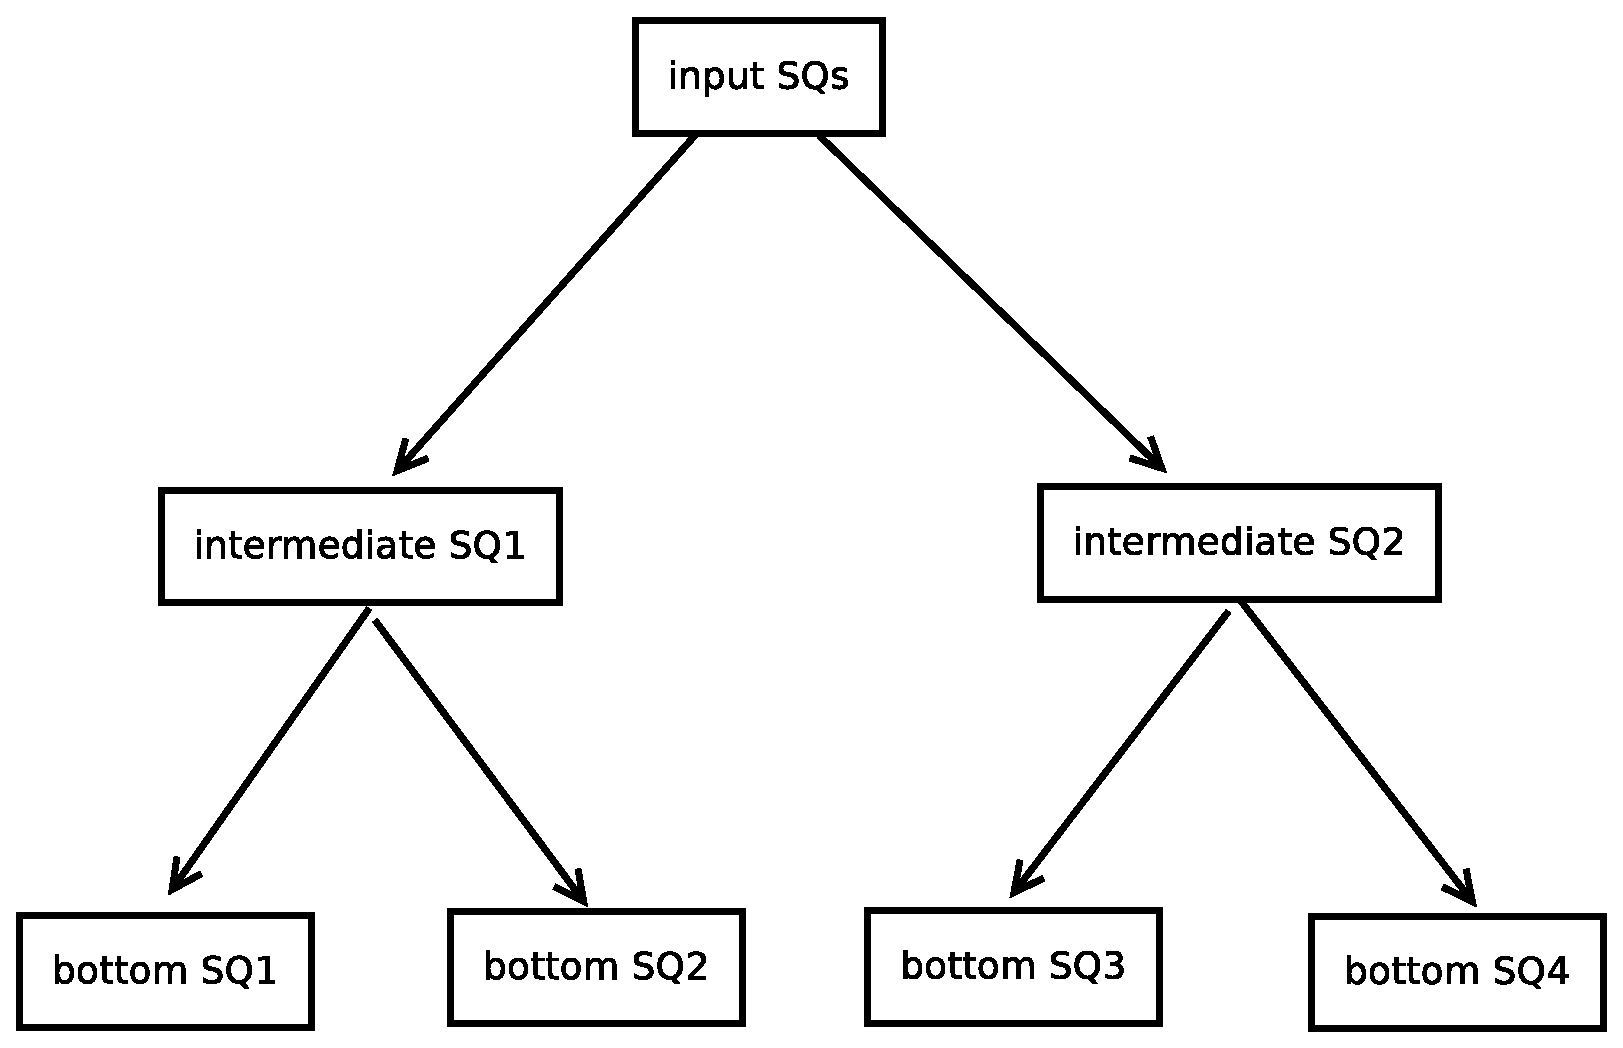
\includegraphics[scale=0.5]{./general_rr.eps}
 % general_rr.eps: 0x0 pixel, 300dpi, 0.00x0.00 cm, bb=0 0 763 487
 \caption{general RR from input shell quartets to bottom shell quartets}
 \label{fig:1}
\end{figure}

The recursive relation is divided into two types. One type is 
vertical recursive relation\ref{vrr}, and the other type is the horizontal
recursive relation\ref{hrr}. In the following content we will discuss each
of them in details.

\subsection{Shell Quartet Path}
%
%
%
\label{rr_sq_path}

For a general LHS shell quartet, it's worthy to note that 
it's RR expansion is usually able to be made on each of 
the shell position. Taking the OS algorithm as an example
\cite{OS1986}, it's RR expansion could be made on each of non-S
shell (the position for expanding the RR is called RR expanding 
position). For example, the OS RR expansion for DPFD ERI shell quartet
could be like below:
\begin{align}
 (\bm{D}P|FD) &\Rightarrow \text{expansion on BRA1} \nonumber \\
 (D\bm{P}|FD) &\Rightarrow \text{expansion on BRA2} \nonumber \\
 (DP|\bm{F}D) &\Rightarrow \text{expansion on KET1} \nonumber \\
 (DP|F\bm{D}) &\Rightarrow \text{expansion on KET2}
\end{align}
It has four possible positions for expansion, and it's able to 
derive the RHS shell quartet based on each possible position.

As a result, it could be imagining that there will be tremendous
choices that is going from the input shell quartets down to the 
bottom shell quartets. Each of such choice is called ``shell quartet 
path'', and every choice is able to give correct integral results.
The only difference between them is their efficiency for integral calculation. 
We note, that among these shell quartet path there's a minimum 
path (here ``MINIMUM'' is defined as the shell quartet path with
minimum integral numbers). How to search this minimum shell quartet
path (it could be also called as optimum shell quartet path), 
will be the most important part for this program.

On the other hand, it's beneficial to know the general property
of the shell quartet path. For a long time, the shell quartet path
is recognized as ``tree'' in terms of data structure\cite{HGP}. However, as 
we can see from the figure \ref{fig:2}, the upper level of shell 
quartets(LHS shell quartets, this could be also called parent nodes) 
may have chance to share the same lower level shell quartets (RHS shell quartets,
and it could be also called children nodes), therefore it violates
the tree definition that each children node could only have one 
parent node. Therefore, the shell quartet path; is actually a ``GRAPH''
rather than ``TREE''. The optimum shell quartet path searching,
is actually graph searching problem. In this program, we use 
the greedy search algorithm to solve the shell quartet searching
problem; the details will be discussed in the following section (see 
section \ref{vrr_sq_search}).

 \begin{figure}[htb]
 \centering
 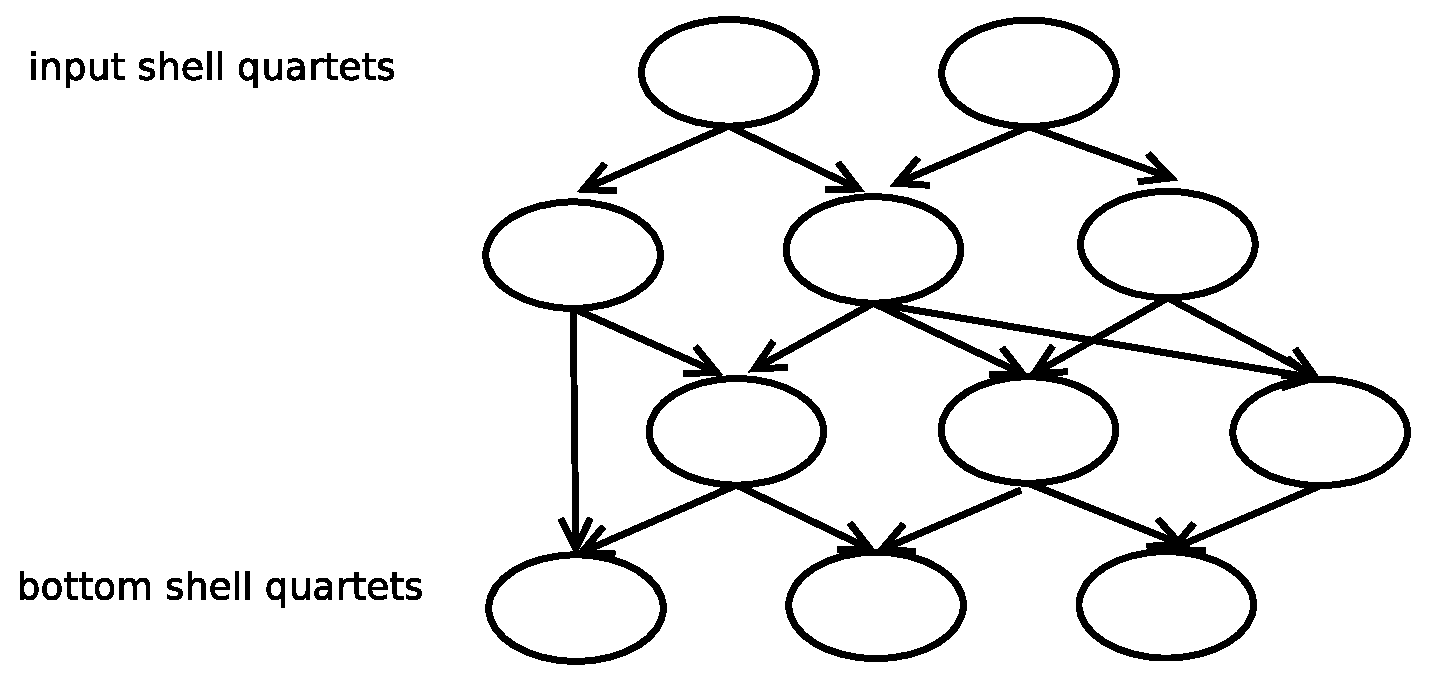
\includegraphics[scale=0.5]{./rr_as_polytree.eps}
 % general_rr.eps: 0x0 pixel, 300dpi, 0.00x0.00 cm, bb=0 0 763 487
 \caption{RR diagram structure as polytree}
 \label{fig:2}
\end{figure}

\subsection{Recursively Generating Integrals}
%
%
%
\label{rr_intereal_gen}
In the last section we have discussed the optimum shell quartet
path searching in general, which is perhaps the most important feature of 
this program. Here we will discuss another feature of RR expansion,
which is to generate integrals in recursive way.

So far most of the integral calculation is on the Cartesian type 
of Gaussian functions\ref{gaussian_function}. 
Compared with the Cartesian Gaussian functions, it also has 
the spherical Gaussian functions whose angular momentum part is  
composed by spherical harmonics rather than the $x^{l}y^{m}z^{n}$. 

However, there's a basic difference between the Cartesian type of 
basis set functions and the spherical type of basis set functions, is 
that the Cartesian basis sets are redundant. For example, Cartesian
D type of shell have 6 basis set functions, and one of them is 
redundant (it's combination could be transformed into S type of 
basis sets). Such feature aspires us to ask this question:
Is there redundancy in integral calculation with the Cartesian
type of basis sets?

For exploring the answer of this question, we derive the final 
integral expressions together with recursive generation. After 
the optimum shell quartet path is acquired, the next step is to
generate the integrals for each given shell quartet on the result
searching path. In this process, each RHS integrals will be 
recursively generated, that is to say; we only pick up the RHS
integrals that appearing on the RR expansion. For example, in 
the following general recursive relation
\begin{align}
 SQ_{LHS}  &= a_{0}SQ_{RHS,0} + a_{1}SQ_{RHS,1} + \cdots \Rightarrow \nonumber \\
 SQ_{RHS,i} &= a^{'}_{0}SQ^{'}_{RHS,0} + a^{'}_{1}SQ^{'}_{RHS,1} + \cdots
\end{align}
for the $SQ_{RHS,i}$ we only pick up the integrals existing on the RR 
expansion. There could be integrals that belongs to $SQ_{RHS,i}$ but 
they does not show up in the RR expansion terms, these integrals
are the ``negligible integrals'' in terms of RR expansion. 

As a result, for each RR expansion on the given shell quartet, the 
result RHS shell quartet may contain less number of integrals than
it's full list. As a consequence, for the integral calculation 
there would be a lot of negligible integrals that it's able to save 
time on the number of integrals which is going to be calculated. 
We note that this feature together with the optimum shell quartet 
path searching, constitutes the most important characters of this 
program.

%%%%%%%%%%%%%%%%%%%%%%%%%%%%%%%%%%%%%%%%%%%%%%%%%%%%%%%%%%%%%%%%%%%%%%%%
\section{Vertical Recursive Relation}
%
%
\subsection{Definition of Vertical Recursive Relation}
%
%
\label{vrr}
Vertical recursive relation(VRR) is a special kind of recursive relation
in RR expression:
\begin{equation}
 SQ_{LHS}  = a_{0}SQ_{RHS,0} + a_{1}SQ_{RHS,1} + \cdots
\end{equation}
In general, the vertical recursive relation is a ``NON-CONVERTIBLE''
RR, which means that it's impossible to find another RR expression that could 
exchange the above RHS shell quartet and LHS shell quartet:
\begin{equation}
 SQ_{RHS} = a_{0}^{'}SQ_{LHS} + \cdots
\end{equation}

To release such non-convertibility character, there must be some 
shell quartet property ``decaying'' from the LHS shell quartet
to the RHS shell quartet. For example, in the ERI of OS framework
the angular momentum is reducing from the LHS to the RHS; and the 
m value is increasing \footnote{see the equation of 39 in \cite{OS1986}
paper}. In the kinetic integral expression the LHS integral
is converted into the kinetic integral with lower total angular momentum
and two body overlap integrals. In the above examples, such RR 
expression are all non-convertible.

\subsection{Optimum Path Searching: How to Form Independent Group}
%
%
\label{vrr_sq_search}

Such non-convertibility character for the VRR expression makes 
the optimum shell quartet path searching applicable. In general,
we adopt the greedy searching technique \footnote{see the 
\url{http://en.wikipedia.org/wiki/Greedy_algorithm} for more 
details} to solve this problem. 

The greedy algorithm can get the best results if the whole searching
area could be decomposed into a series of local areas with descending 
weights, as shown in figure \ref{fig:3} (in \ref{fig:3} the size 
of the circle indicates its weights):

 \begin{figure}[htb]
 \centering
 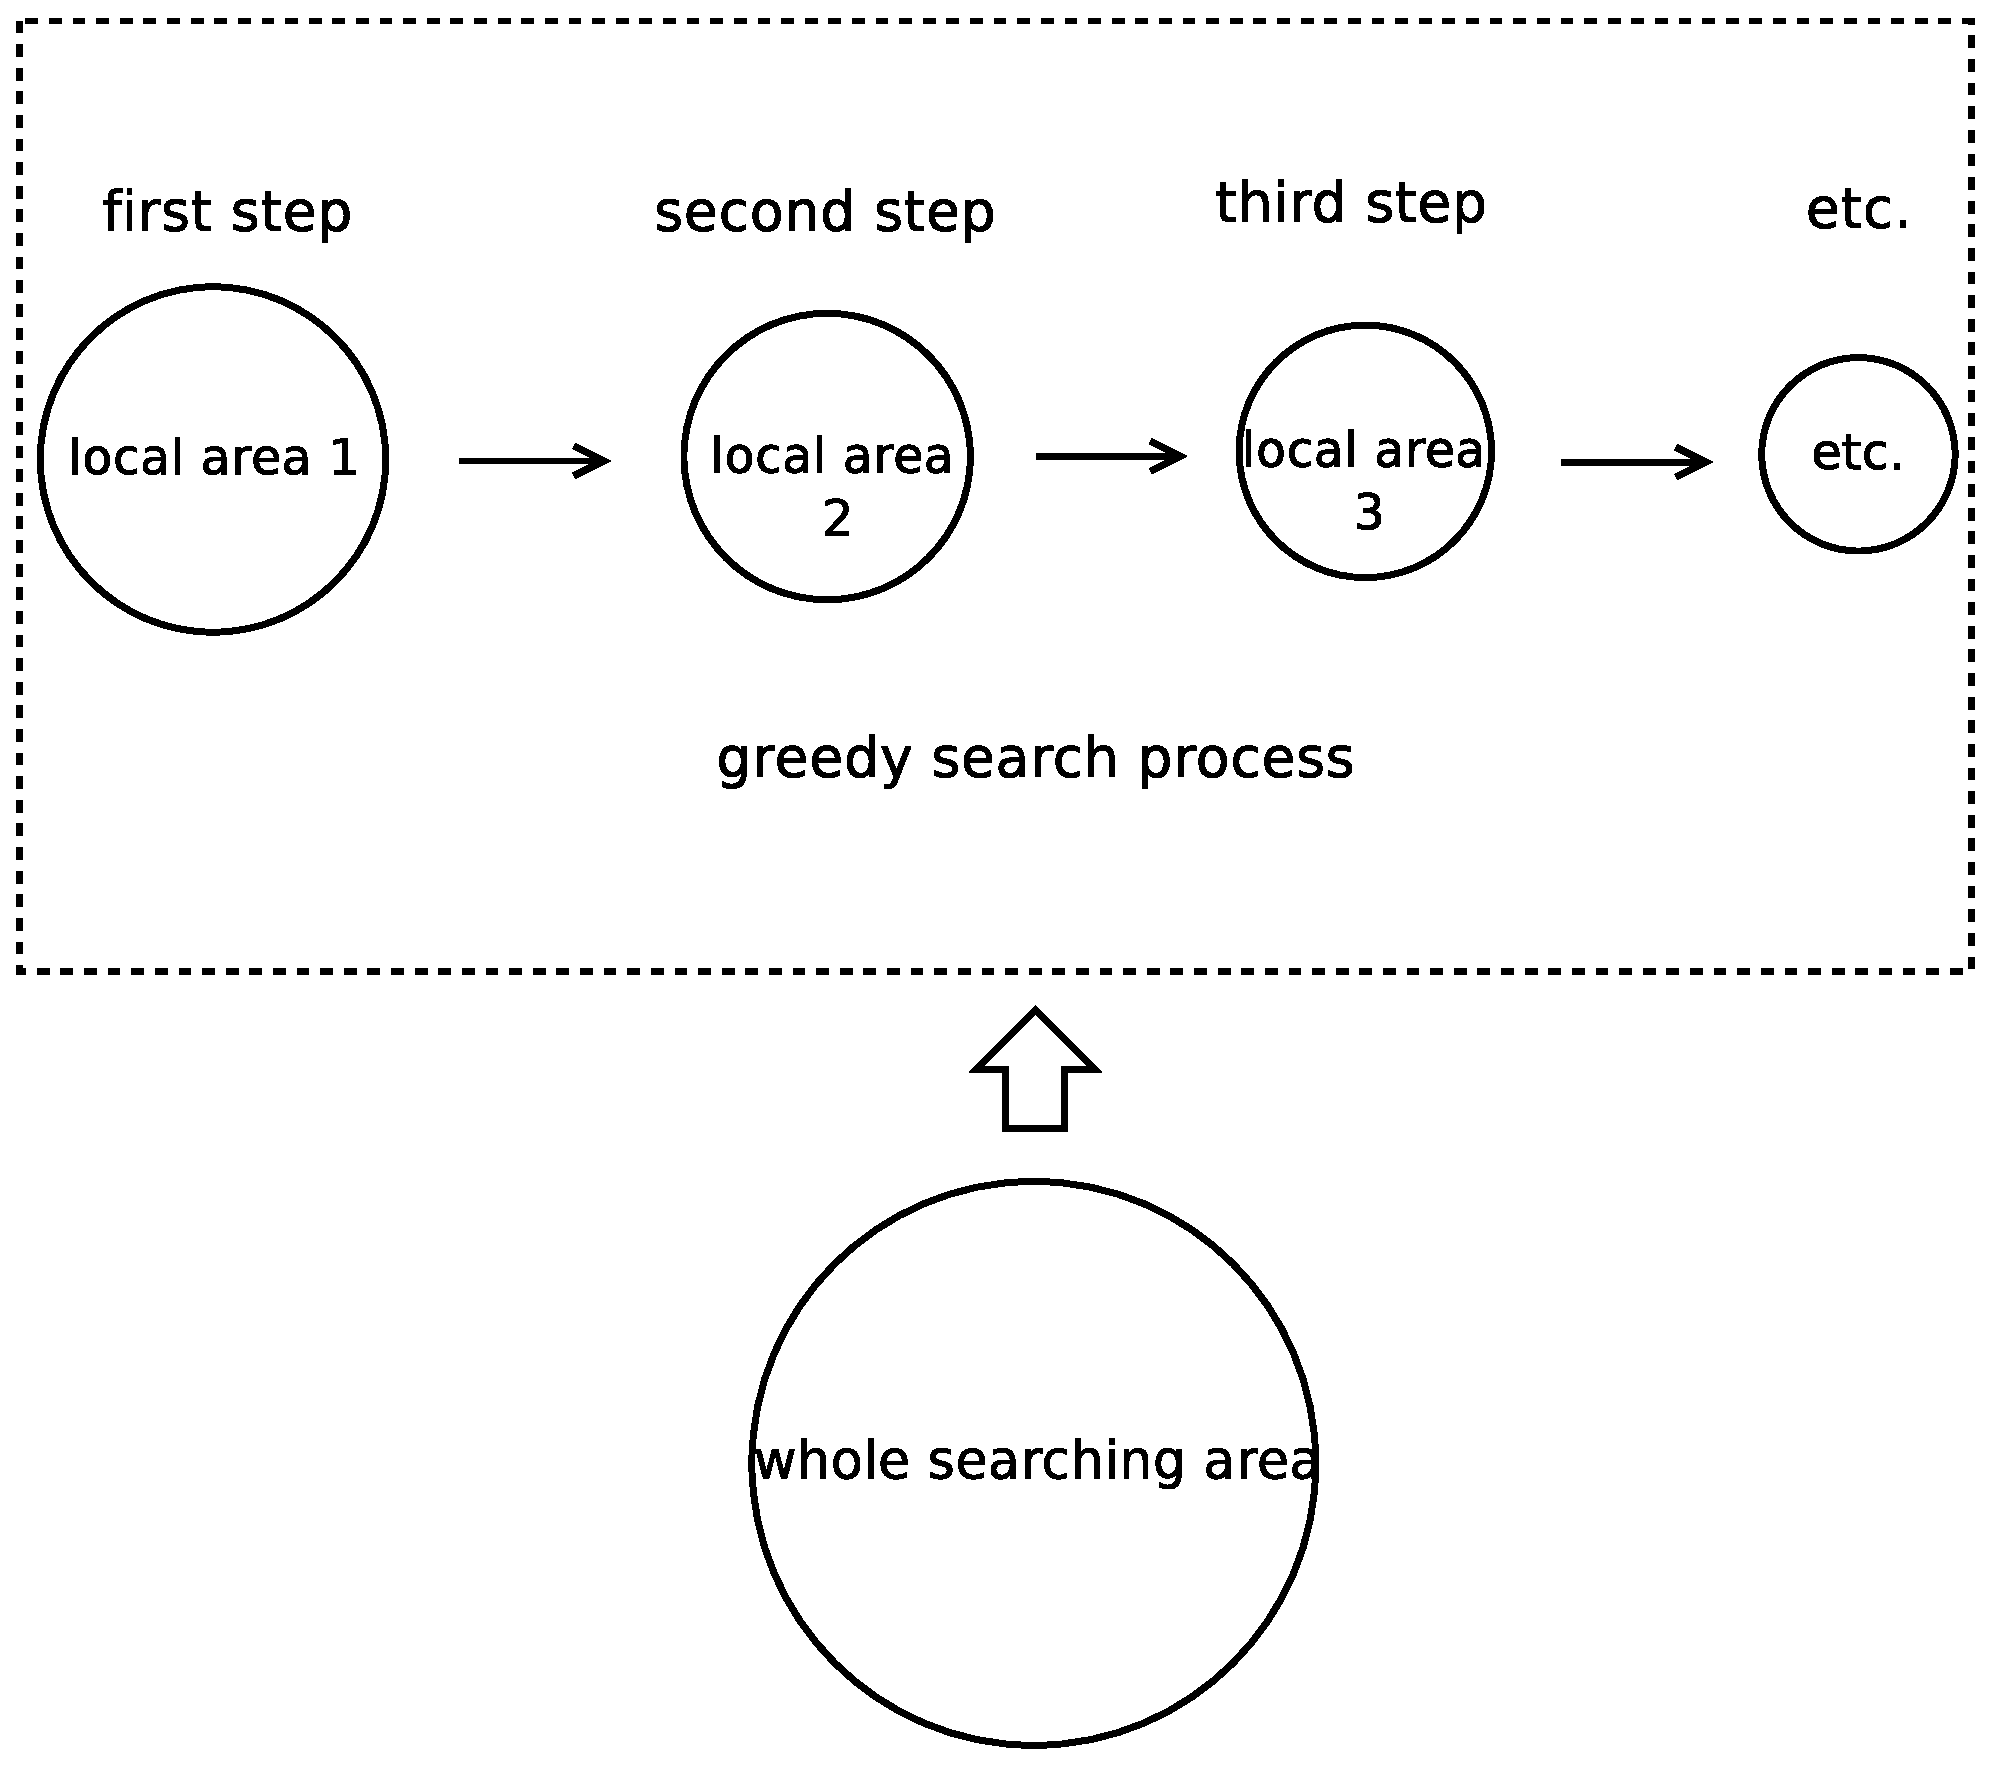
\includegraphics[scale=0.4]{./greedy.eps}
 % general_rr.eps: 0x0 pixel, 300dpi, 0.00x0.00 cm, bb=0 0 763 487
 \caption{general greedy searching algorithm}
 \label{fig:3}
\end{figure}

The best result for greedy searching algorithm could be achieved 
if the dividing local areas are independent with each other, and the
weights are smoothly descending as the greedy searching steps move
forward.

How to achieve it in the optimum shell quartet path searching?
We note, that according to the decaying shell quartet properties 
appearing in the VRR expression, it's possible to wrap the shell
quartets into groups; and different groups have no overlap with
each other - which is to say, different groups are independent with 
each other in terms of VRR process. The optimum weight search will
be carried out for each of the group.

Let's go to an example for more details. Suggest we have a bunch of 
ERI shell quartets, namely $sq_{1}$, $sq_{2}$ etc. until to $sq_{n}$.
The recursive relation for ERI under OS framework is given below:
\begin{equation}
 \begin{split}
((a+\iota_{i})b|cd)^{(m)} &= (P_{i} - A_{i})(ab|cd)^{(m)} +
\left(W_{i} -P_{i}\right)(ab|cd)^{(m+1)} \\
&+\frac{N_{i}(A)}{2\epsilon}\left(((a-\iota_{i})b|cd)^{(m)}-\frac{\rho}{
\epsilon }((a-\iota_{i})b|cd)^{(m+1)}\right)  \\
&+\frac{N_{i}(B)}{2\epsilon}\left((a(b-\iota_{i})|cd)^{(m)}-\frac{\rho}{
\epsilon }(a(b-\iota_{i})|cd)^{(m+1)}\right)  \\
&+\left(\frac{N_{i}(C)}{2}\right)\frac{1}{\epsilon+\eta}
(ab|(c-\iota_{i})d)^{(m+1)} \\
&+\left(\frac{N_{i}(D)}{2}\right)\frac{1}{\epsilon+\eta}
(ab|c(d-\iota_{i}))^{(m+1)}
\end{split}
\label{OS_ERI_result}
\end{equation}
$\iota_{i}$ means an increasing of angular momentum on the $i$th direction (i
could be x, y or z)\footnote{For more understanding of the variables 
appearing on this VRR, you can refer to the material of \cite{OS1986}}. 

Here we can see, that the total angular momentum on the RHS shell quartets are 
$L-1$ or $L-2$ if the total angular momentum for given LHS shell quartet is $L$.
On the other hand, the M value on the RHS is also increasing. All in all, the 
total angular momentum as well as the M value, are the key shell properties
we consider to form the group used in searching process for ERI.

The next step, is to consider that how can we form the independent group.
For an arbitrary total angular momentum L and M value on LHS shell quartet, 
it's easy to see that only the shell quartets with property pairs of (L,M), 
(L,M+1), (L-1,M) and (L-1,M+1) can have the same RHS shell quartet terms compared 
with the LHS shell quartets. Therefore, we note that the shell quartets with 
property pairs of (L,M), (L,M+1), (L-1,M) and (L-1,M+1) will form a 
group, in which the main shell quartet list (these shell quartets who
match th property pair of (L,M), the other shell quartets is called 
appended shell quartet list) is able to form a ``completely'' self-closed 
RR searching path. This main shell quartet list is independent with the 
shell quartets from other groups in terms of the VRR shell quartet path forming.

Here it's worthy to note that for the shell property pair of (L-2,M) and (L-2,M+1),
they are not going to be the criteria of forming the shell quartet group. This 
is because for the shell quartet with total angular momentum $L-2$, if they 
appear on the LHS the RHS shell quartet will have the angular momentum of L-3 or 
L-4, which has no overlap with RHS shell quartets shown above.

Therefore the general searching process for ERI is like below:
\begin{verbatim}
set up the result shell quartet archive and unsolved
shell quartet archive;

push the input shell quartet list into the unsolved
shell quartet archive;

loop over M value (from maximum to 0):
  loop over L (from Lmax to 0):
    for each M and L form main shell quartet list and 
    appended shell quartet list from unsolved shell
    quartet archive;
    do greedy search to the both of the two lists so
    that to find the best RR expanding position for 
    the main shell quartet list;
    push the main shell quartet list to the result
    shell quartet archive;
    form the new unsolved shell quartet (RHS shell 
    quartets) from the main shell quartet list 
    according to the new RR position;
    push the new unsolved shell quartets into the 
    unsolved shell quartet archive;
    clean the unsolved shell quartet archive;
  end loop over L
end loop over M
\end{verbatim}

Now a general searching procedure has been established. Given by 
such independent group forming technique, the whole shell quartet
path is able to be divided into different local groups. Here inside
the shell quartet path searching, the weight for each shell quartet
is determined by its number of integrals (here we use it's full integral
numbers instead of the recursively generated integral numbers. The 
recursively generated integral numbers could be only known in the real
RR step, but the RR path searching step is the prior step). Hence it could 
be well expected that as the searching process is carrying on, the weight
of the shell quartets is also descending. Hence it could be expected the 
result shell quartet path generated by such procedure will be in good 
approximation with the real optimum shell quartet path.

\subsection{Optimum Path Searching: Greedy Algorithm Application}
%
%
\label{vrr_sq_search2}

Now the problem has been transformed to the situation that for a group of 
selected shell quartets, how can we perform the greedy search algorithm.

In general sense, the greedy searching procedure is simple. For each shell
quartet in the group, we will find it's every possible RR expansions and 
record it. Then we will search all possible combinations for RR expansions 
so that to find the best position arrangement who gives the minimum 
total integral numbers. Suggest we have $n$ shell quartets, and each
shell quartet $sq_{i}$ has $m_{i}$ ($m_{i} \leq 4$) possible RR expansions;
then the possible combination number would be $\prod_{i=1}^{n} m_{i}$.

In the greedy search procedure, all of RHS shell quartets (those who appear
in the possible RR expansion) will go through two steps sort-out. One
step is called ``horizontal comparisons'', in which all of RHS shell quartet
given in this combination will be sorted to make sure that no one is counted 
more than once. This is because that the LHS shell quartets may generate 
the same RHS terms, and these terms should be counted only once.

The other step is called ``historical comparisons''. It means that before 
the practical greedy search procedure, each of the RHS shell quartet will be 
examined by comparing with the result shell quartet archive and unsolved 
shell quartet archive. If the possible RHS shell quartet appears in either 
of the two archives, then it's status will be indicated as ``OLD''; and the 
old shell quartets will not be counted in the greedy search procedure.

The two steps of sort-out may cause someone to prompt a question: is it safe
to do this? In the later section (see \ref{sort_shell_quartet_vrr}) we will
explore more details for this question.

\subsection{Building Vertical Recursive Relation}
%
%
\label{vrr_build}
After the optimum shell quartet path is got, then it's possible to 
build the whole VRR based on the given path. The general procedure
is like below:
\begin{verbatim}

form the initial unsolved shell quartet list and it's 
corresponding unsolved integral list from input shell 
quartets;

enter into building loop:
  loop over shell quartet in unsolved list:
    do we have it in result?
    if yes, we do updating work rather than
    building work;
  end loop
  set up tmp unsolved shell quartet list and 
  tmp unsolved integral list;
  loop over shell quartet in unsolved list:
    do we go to build a new RR result?
    if yes we do it, and push it into the 
    result list;
    extracting the RHS shell quartets and 
    new unsolved integral list from this 
    newly created RR result;
    push them into the tmp list;
  end loop
  if tmp unsolved shell quartet list does 
  not contain anything, then it's time 
  to break out the loop;
  else we switch the tmp list with the 
  input list, go over again;
end loop
\end{verbatim}

In such treatment, it's possible that we may miss some RHS integrals
that in the practical code, these RHS integrals do not defined in its 
shell quartet section. To avoid this, after the building procedure
it's necessary to perform the ``completeness check'' procedure. 
Basically the completeness check procedure is similar to the above.
For the given arbitrary undetermined integrals, we will recursively
update them in the result shell quartet list until all of them are 
found to be defined.

\subsection{Sorting Shell Quartets in Vertical Recursive Relation}
%
%
\label{sort_shell_quartet_vrr}

After all of shell quartets and it's integral are built, there's 
an question that they are needed to be printed out in ``CORRECT''
order. What is the correct order? It means that each of the 
shell quartets must be defined first (appearing on the LHS), 
then it could be appearing on the RHS.

For the vertical recursive relation, the non-convertibility character
guarantees that there's an unique `` less than '' order to arrange
all of VRR results. This is because the shell quartet properties 
are decaying from LHS to RHS, therefore in the following corrected 
shell quartet chain:
\begin{equation}
 sq_{input} \Rightarrow sq_{1} \Rightarrow sq_{2} \Rightarrow \dots
 \Rightarrow sq_{bottom}
\end{equation}
every shell quartet will be placed in correct order.

Such property also answer the question given in section \ref{vrr_sq_search2}.
For all of possible shell quartets in the result shell quartet path,
they could be divided into different ``chains'' like above. For 
each chain, the left hand side is depending on the right hand side 
until the bottom shell quartets are met. Given by the existing 
unique order provided by decaying shell quartet property, all 
the shell quartets on each chain could be correctly placed. Therefore,
we do not need to worry whether the ``OLD'' shell quartet is defined 
or not. As long as the ``OLD'' shell quartet is in RHS of the given
shell quartet, both of them will be correctly placed.

%%%%%%%%%%%%%%%%%%%%%%%%%%%%%%%%%%%%%%%%%%%%%%%%%%%%%%%%%%%%%%%%%%%%%%%%
\section{Horizontal Recursive Relation}
%
%
\subsection{Definition of Horizontal Recursive Relation}
%
%
\label{hrr}

The horizontal recursive relation\footnote{``A method for two-electron Gaussian 
integral and integral derivative evaluation using recurrence relations'', 
The Journal of chemical physics, Vol. 89, Page 5777, 1988} provides a new method 
to transform the integral in horizontal level (HRR expression):
\begin{align}
\label{HRR_expression}
 (a(b+\iota_{i})|cd)^{(m)} &= ((a+\iota_{i})b|cd)^{(m)} + 
(A_{i} - B_{i})(ab|cd)^{(m)} \nonumber \\
 ((a+\iota_{i})b|cd)^{(m)} &= (a(b+\iota_{i})|cd)^{(m)} - 
(A_{i} - B_{i})(ab|cd)^{(m)}
\end{align}
The example here is given for ERI, for overlap integrals, nuclear attraction
integral etc. it's able to find the similar HRR expressions. 

The HRR expression has the following features:
\begin{itemize}
 \item the bra and ket sides are independent with each other;
 \item the RR expression is convertible between RHS and LHS;
 \item only the angular momentum is involved into the HRR expansion, 
 no other shell quartet properties are involved anymore
\end{itemize}

Here it's worthy to discuss more about the convertibility for HRR. 
In \ref{HRR_expression}, the second equation is just the convertible
expression of first equation, and vice versa. Such convertibility
in HRR brings a consequence that the searching technique is not 
applicable here anymore. If the minimum searching technique 
is applied, the situation below could happen: 
\begin{equation} 
A \Rightarrow B \Rightarrow \dots \Rightarrow A
\end{equation}
In the minimum search process since the ``OLD'' shell quartets (see 
\ref{vrr_sq_search2} for the interpretation of ``OLD'' meaning) 
is always not counted in, therefore it's possible to form such a loop
in the result shell quartet path, so to screw up the whole thing. 
Therefore, to perform HRR shell quartet search it's always with a 
pre-defined position. Since the HRR can only have two possible 
positions, therefore we will perform the shell quartet path for each
position, then pick up the one with smallest weight.

\subsection{Building Horizontal Recursive Relation}
%
%
\label{build_hrr}

After the shell quartet path is gotten, the building of HRR procedure 
is carried out in the same way as shown in VRR part (see \ref{vrr_build}).
So as the completeness checking procedure.

Because of the convertibility character of HRR, in general you can not
do the sorting to the HRR results. However, it's possible to define
a sorting order so that to make sure the LHS shell quartet is following
the RHS shell quartet definition.


